\newpage
\section{Explore second-order effects (Body effect, Channel-length modulation)}

\subsection{NMOS}

\begin{figure}[H]
	\centering
	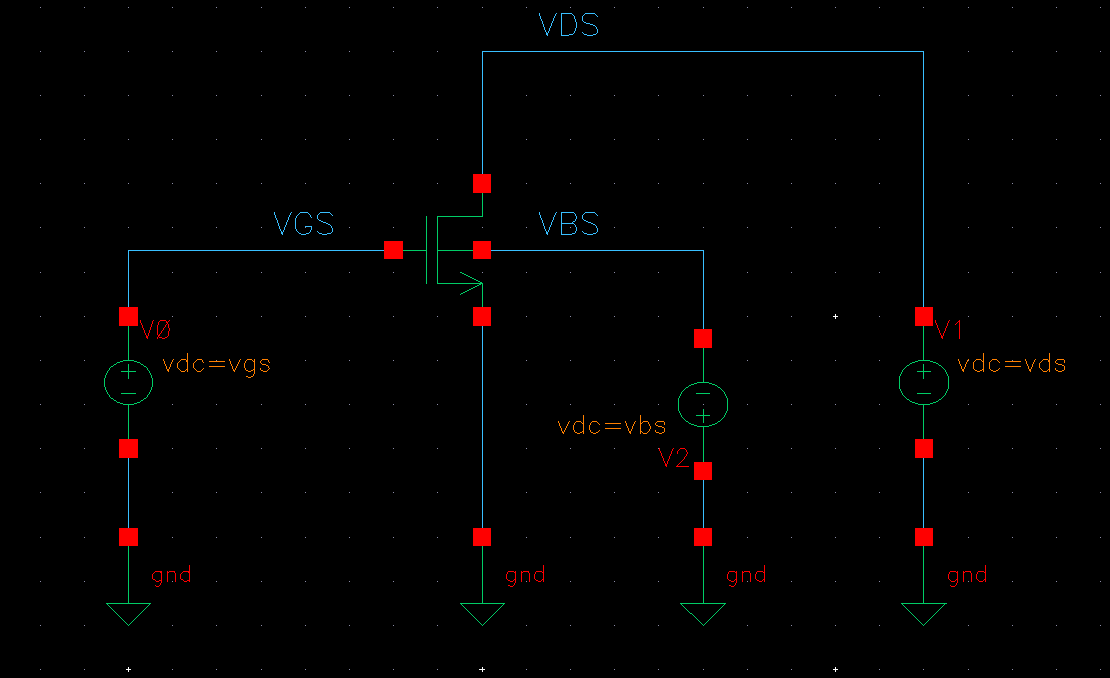
\includegraphics[width = 0.6\linewidth]{sections/pic/EX3_NMOS_schematic.png}
	\caption{Testbench NMOS\_VTG for experiment 3.}
	\label{f_ex3NMOS-schematic}
\end{figure}

\itemmini{Draw curves $I_{D}$ vs $V_{GS}$ @ $V_{DS} = 1V$, $V_{SB} = [0.1, 0.55, 0.9] V$, and sweeping $V_{GS} = [0, 1.5]V$ with step $10mV$.}

\begin{figure}[H]
	\centering
	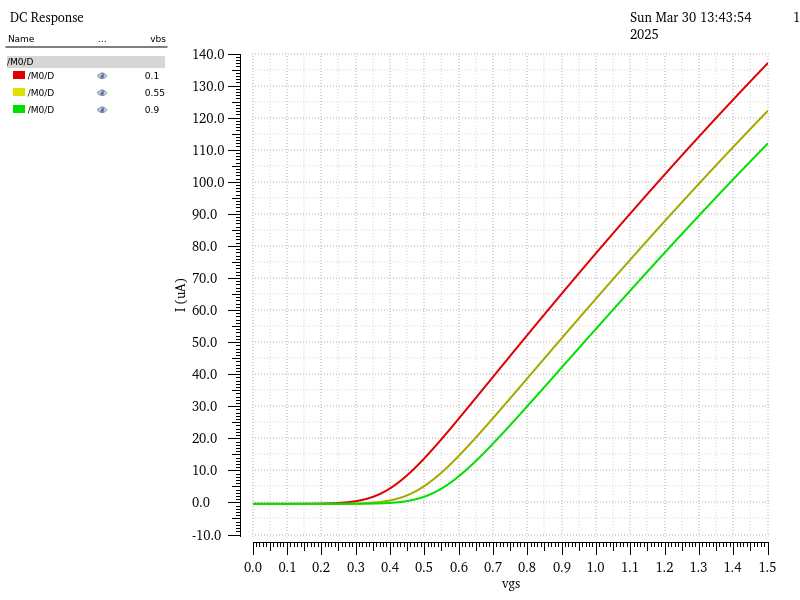
\includegraphics[width=.6\linewidth]{sections/pic/EX3_NMOS_Id&Vgs(Vds=0_1)(w)(l).png}
	\caption{$I_{D}$ vs $V_{GS}$ @ $V_{DS} = 1V$, $V_{SB} = [0.1, 0.55, 0.9] V$, and sweeping $V_{GS} = [0, 1.5]V$ with step $10mV$.}
	\label{f_EX3_NMOS_Id&Vgs(Vds=0_1)(w)(l)}
\end{figure}

\begin{discussion}
	\item When \( V_{SB} \) increases, meaning \( V_{B} \) becomes more negative, the threshold voltage \( V_{TH} \) increases. We can see this phenomenon clearly in the figure. The reason for this is the body effect.  
	
	\[ V_t = V_{t0} + \gamma \left( \sqrt{\phi_{s} + V_{SB}} - \sqrt{\phi_{s}} \right) \]
\end{discussion}

\itemmini{Draw curves $I_{D}$ vs $V_{DS}$ @ $V_{GS} = 1V$, $V_{SB} = [0.1, 0.55, 0.9] V$, and sweeping $V_{DS} = [0, 1.5] V$ with step $10mV$.}

\begin{figure}[H]
	\centering
	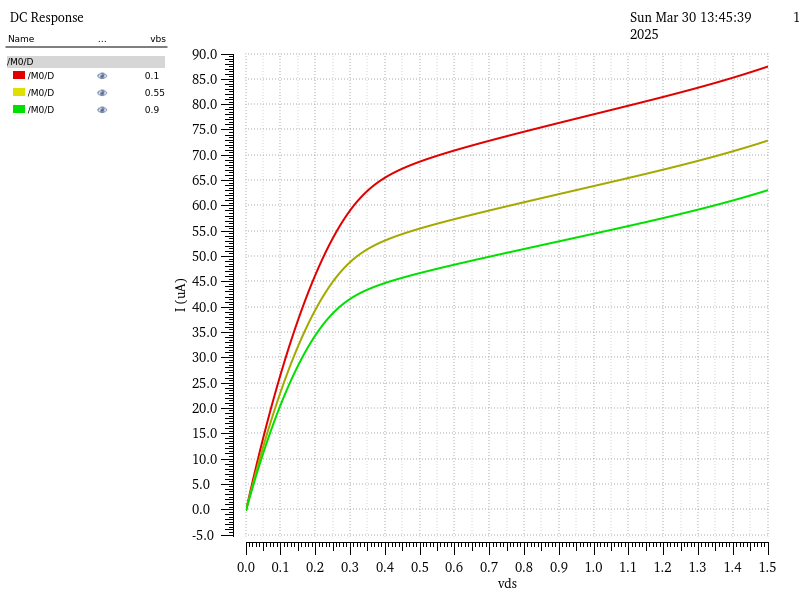
\includegraphics[width=.6\linewidth]{sections/pic/EX3_NMOS_Id&Vds(Vgs=0_1)(w)(l).png}
	\caption{$I_{D}$ vs $V_{DS}$ @ $V_{GS} = 1V$, $V_{SB} = [0.1, 0.55, 0.9] V$, and sweeping $V_{DS} = [0, 1.5] V$ with step $10mV$.}
	\label{f_EX3_NMOS_Id&Vds(Vgs=0_1)(w)(l)}
\end{figure}

\begin{discussion}
	\item With a higher \( V_{TH} \) as \( V_{SB} \) increases, the gate overdrive voltage \( V_{GT} \) becomes smaller. In general, the \( I_{DS} \)-\( V_{DS} \) characteristics tend to be lower and smaller as \( V_{SB} \) increases. 
	
	\[ I_{DS} = \dfrac{\beta}{2} V_{GT}^{2} \left( 1 + \dfrac{V_{DS}}{V_{A}} \right)\]
\end{discussion}

\subsubsection{Measure $\lambda$}
\textbf{Note:} Take points in the saturation region.\\

Draw the curves for $I_{D}$ vs $V_{DS} = [0, 1.5] V$ with a step of $10\text{mV}$, for two values of $V_{GS} = \{0.5, 0.75\} V$ and $V_{BS} = 0V$ for this simulation.\\

\itemmini{For the NMOS transistor with $(Wz/L) = (90n/50n)$.}

\begin{figure}[H]
	\centering
	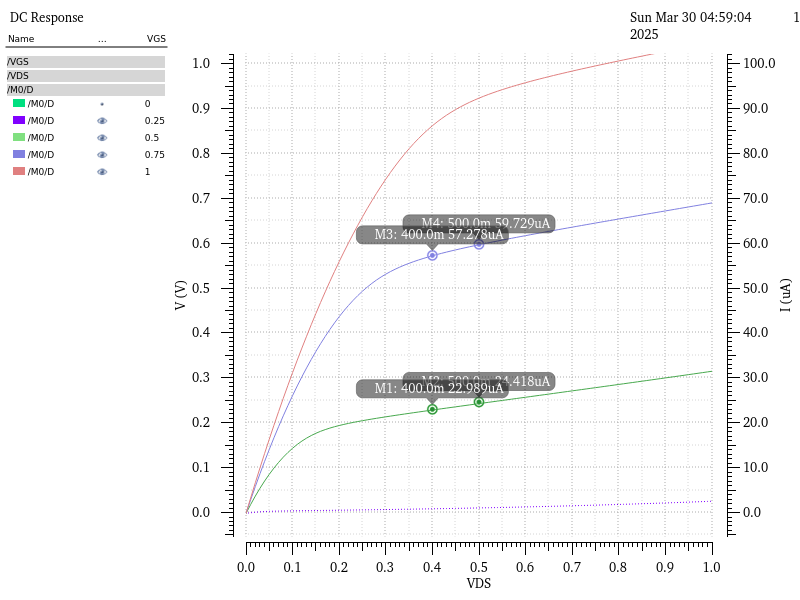
\includegraphics[width=0.6\linewidth]{sections/pic/EX3_NMOS_lambda_(w_l)(90_50).png}
	\caption{$I_{DS}$ vs $V_{DS}$ with a step of $10mV$ for two value of $V_{GS} = \{0.5, 0.75\} V$, the NMOS with $(W/L) = (90n/50n)$}
	\label{f_EX3_NMOS_lambda_(w_l)(90_50)}
\end{figure}

\[ \lambda = \dfrac{I_{D2} - I_{D1}}{I_{D1} V_{DS2} - I_{D2} V_{DS1}} \]

With $V_{GS} = 0.5$, we have:
\[ \lambda = \dfrac{I_{D2} - I_{D1}}{I_{D1} V_{DS2} - I_{D2} V_{DS1}} = \dfrac{(24.42 - 22.99)\times 10^{-6}}{22.99\times 10^{-6}\times 0.5 - 24.42 \times 10^{-6} \times 0.4 }  = 0.82\]

With $V_{GS} = 0.75$, we have:
\[ \lambda = \dfrac{I_{D2} - I_{D1}}{I_{D1} V_{DS2} - I_{D2} V_{DS1}} = \dfrac{(59.73 - 57.28)\times 10^{-6}}{57.28\times 10^{-6}\times 0.5 - 59.73 \times 10^{-6} \times 0.4 }  = 0.52\]

We observe that $\lambda(0.5) > \lambda(0.75)$. This implies that when $V_{GS}$ is low, the stability of $I_{DS}$ in the saturation region is poorer.\\ 

\itemmini{For the NMOS transistor with $(W/L) = (120n/60n)$.}

\begin{figure}[H]
	\centering
	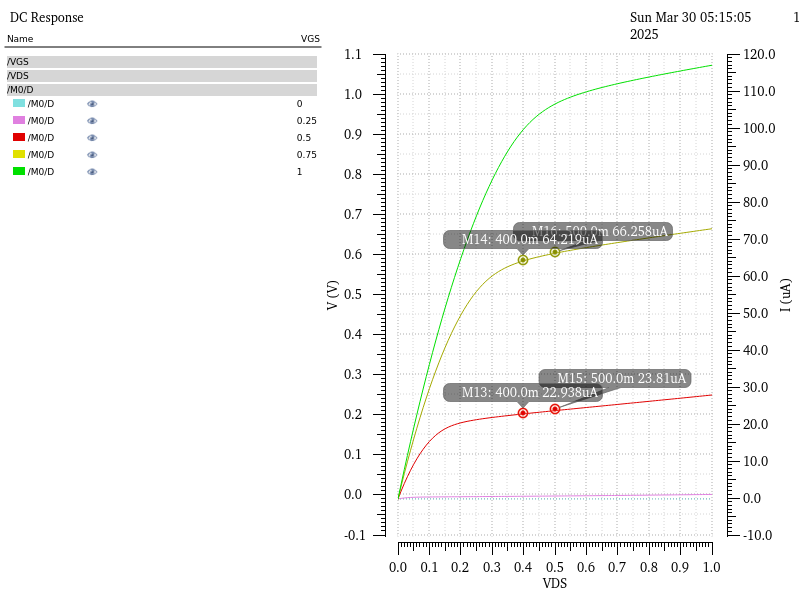
\includegraphics[width=.6\linewidth]{sections/pic/EX3_NMOS_lambda_(w_l)(120_90)(vgs_0_5).png}
	\caption{$I_{DS}$ vs $V_{DS}$ with a step of $10mV$ for two value of $V_{GS} = \{0.5, 0.75\}$, the NMOS with $(W/L) = (120n/60n)$}
	\label{f_EX3_NMOS_lambda_(w_l)(120_90)(vgs_0_5)}
\end{figure}

With $V_{GS} = 0.5$, we have:
\[ \lambda = \dfrac{I_{D2} - I_{D1}}{I_{D1} V_{DS2} - I_{D2} V_{DS1}} = \dfrac{(23.81 - 22.94)\times 10^{-6}}{22.94\times 10^{-6}\times 0.5 - 23.81 \times 10^{-6} \times 0.4 }  = 0.44 \]

With $V_{GS} = 0.75$, we have:
\[ \lambda = \dfrac{I_{D2} - I_{D1}}{I_{D1} V_{DS2} - I_{D2} V_{DS1}} = \dfrac{(66.26 - 64.22)\times 10^{-6}}{64.22 \times 10^{-6}\times 0.5 - 66.25 \times 10^{-6} \times 0.4 }  = 0.37 \]

Thus, for NMOS transistors with smaller technologies, $\lambda$ increases. This is because, as $L$ decreases, the \textit{Short Channel Effect (SCE)} becomes more pronounced, enhancing the dependence of $I_{DS}$ on $V_{DS}$. Consequently, the channel length modulation factor $\lambda$ increases, indicating reduced stability of $I_{DS}$.

\itemmini{Usingtool}
\begin{figure}[H]
	\centering
	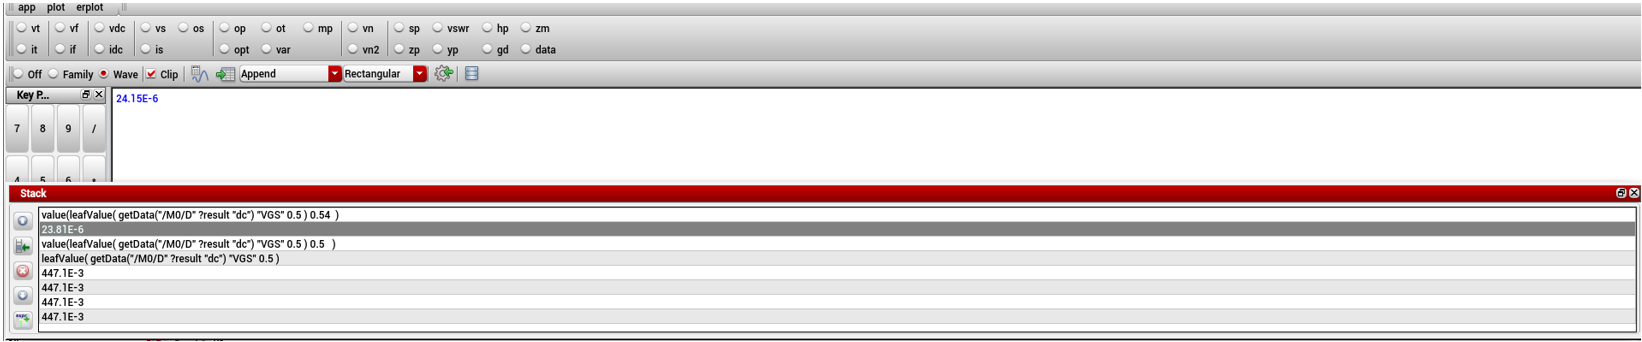
\includegraphics[width=0.8\linewidth]{sections/pic/EX3_NMOS_tool_cal_lambda.png}
	\caption{Use a tool to calculate $\lambda$.}
	\label{f_EX3_NMOS_tool_cal}
\end{figure}

\subsubsection{Measure $V_{Th0}$}
\[ V_{Th} = \dfrac{V_{GS1} - V_{GS2}\sqrt{\dfrac{I_{DS1}}{I_{DS2}}}}{1 - \sqrt{\dfrac{I_{DS1}}{I_{DS2}}}} \]

\itemmini{For the NMOS transistor with $(W/L) = (90n/50n)$.}

\begin{figure}[H]
	\centering
	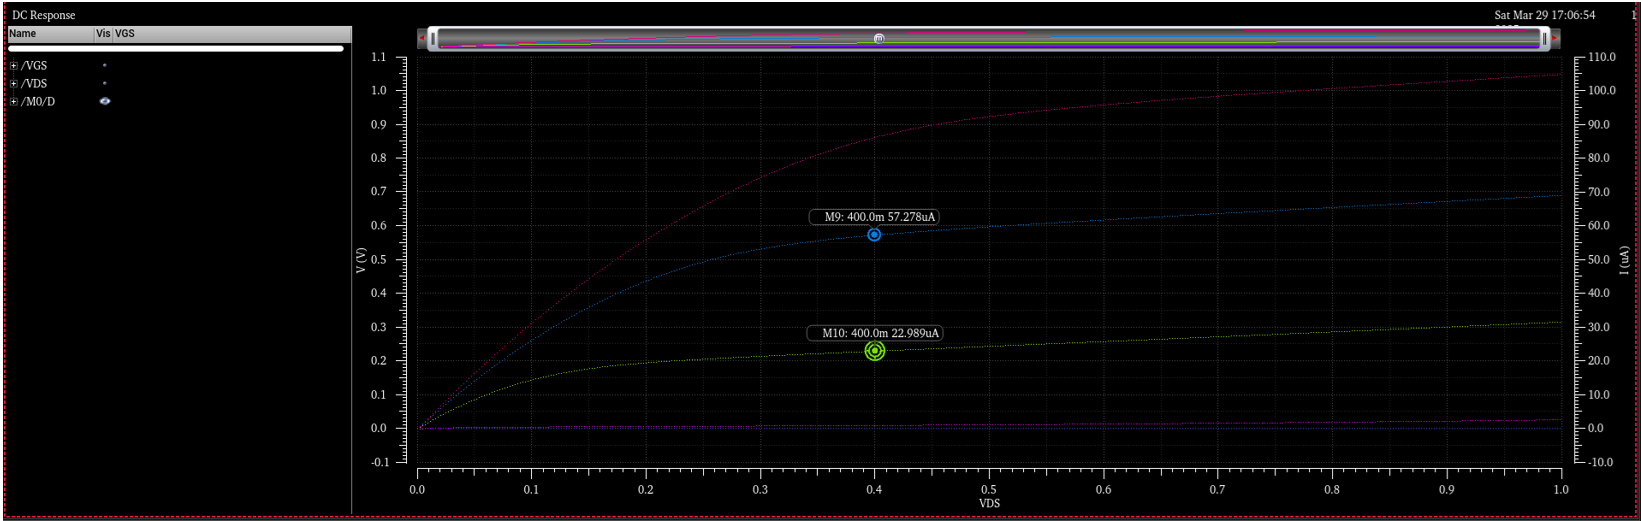
\includegraphics[width=.6\linewidth]{sections/pic/EX3_NMOS_vth0_(w_l)(90_50).png}
	\caption{$I_{DS}$ vs $V_{DS}$ with step $10mV$ with $(W/L) = (90n/50n)$}
	\label{f_EX3_NMOS_vth0_(w_l)(90_50)}
\end{figure}

\[ V_{Th0} = \dfrac{V_{GS1} - V_{GS2}\sqrt{\dfrac{I_{DS1}}{I_{DS2}}}}{1 - \sqrt{\dfrac{I_{DS1}}{I_{DS2}}}} = \dfrac{0.75 - 0.5\times \sqrt{\dfrac{57.28\times 10^{-6}}{22.99\times 10^{-6}}}}{1 - \sqrt{\dfrac{57.28\times 10^{-6}}{22.99\times 10^{-6}}}} = 0.07(V)\]

\itemmini{For the NMOS transistor with $(W/L) = (120n/60n)$.}

\begin{figure}[H]
	\centering
	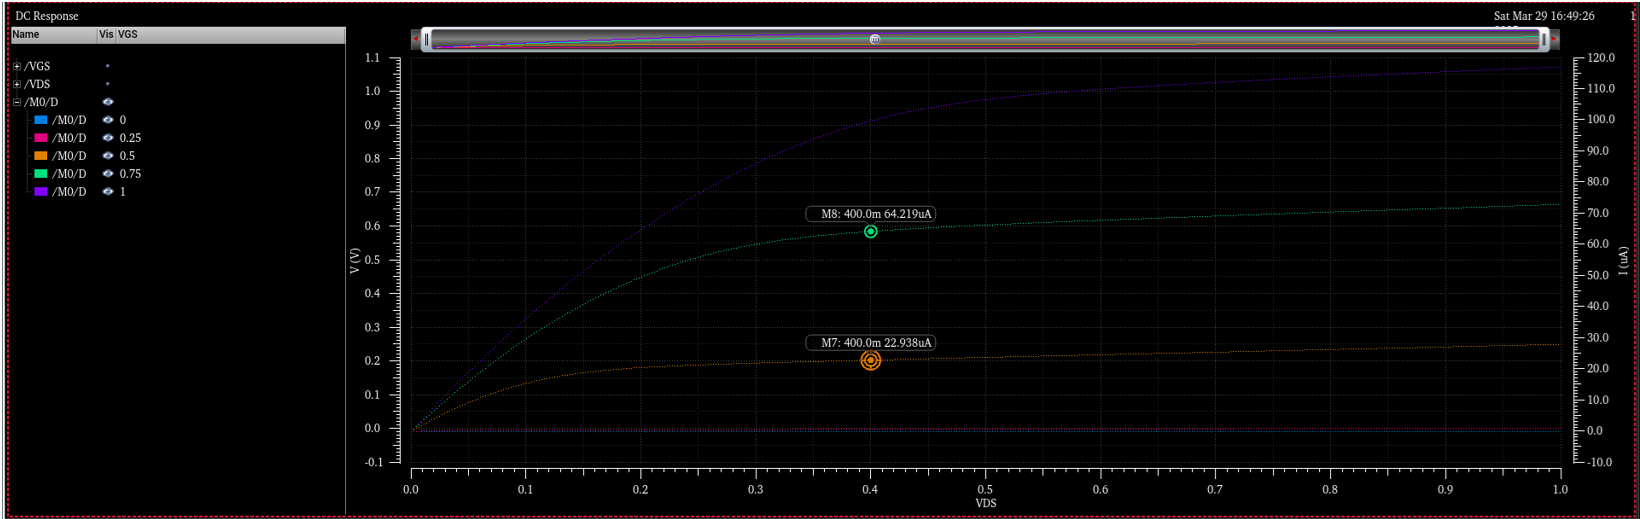
\includegraphics[width=.6\linewidth]{sections/pic/EX3_NMOS_vth0_(w_l)(120_60).png}
	\caption{$I_{DS}$ vs $V_{DS}$ with step $10mV$ with $(W/L) = (120n/60n)$}
	\label{f_EX3_NMOS_vth0_(w_l)(120_60)}
\end{figure}

\[ V_{Th0} = \dfrac{V_{GS1} - V_{GS2}\sqrt{\dfrac{I_{DS1}}{I_{DS2}}}}{1 - \sqrt{\dfrac{I_{DS1}}{I_{DS2}}}} = \dfrac{0.75 - 0.5\times \sqrt{\dfrac{64.22\times 10^{-6}}{22.94\times 10^{-6}}}}{1 - \sqrt{\dfrac{64.22\times 10^{-6}}{22.94\times 10^{-6}}}} = 0.13(V)\] 


When the $W/L$ ratio changes, $V_{TH}$ can be affected due to the \textit{SCE - Short Channel Effect}.

When $L$ decreases (in the case of NMOS $90n/50n$), $V_{TH}$ tends to decrease due to the \textit{Drain-Induced Barrier Lowering (DIBL)} effect.

When $L$ increases (in the case of NMOS $120/60n$), $V_{TH}$ is higher because the short channel effect becomes less pronounced.

\subsubsection{Measure $\gamma$}

\itemmini{For the NMOS transistor with $(W/L) = (90n/50n)$ and $V_{BS} = 0.5$.}

\begin{figure}[H]
	\centering
	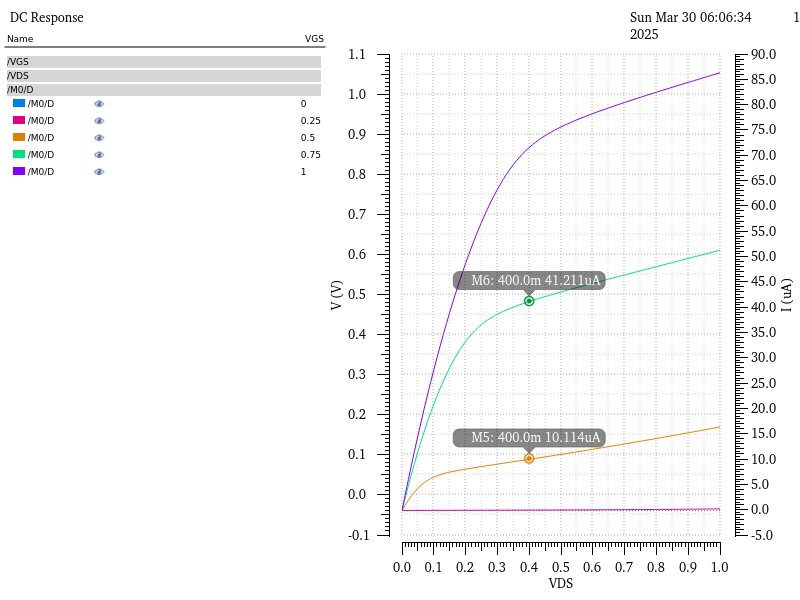
\includegraphics[width=.6\linewidth]{sections/pic/EX3_NMOS_gamma_(w_l)(90_50).png}
	\caption{$I_{DS}$ vs $V_{DS}$ with step $10mV$ with $(W/L) = (90n/50n)$}
	\label{f_EX3_NMOS_gamma_(w_l)(90_50)}
\end{figure}

\[ V_{Th} = \dfrac{V_{GS1} - V_{GS2}\sqrt{\dfrac{I_{DS1}}{I_{DS2}}}}{1 - \sqrt{\dfrac{I_{DS1}}{I_{DS2}}}} = \dfrac{0.75 - 0.5\times \sqrt{\dfrac{41.21\times 10^{-6}}{10.11\times 10^{-6}}}}{1 - \sqrt{\dfrac{41.21\times 10^{-6}}{10.11\times 10^{-6}}}} = 0.25(V)\] 


We have, $2\phi F = 0.7 \gamma$:

\[ \gamma = \dfrac{V_{Th} - V_{Th0}}{\sqrt{|2\phi_{F}| + |V_{BS} } - \sqrt{|2\phi_{F}}} = \dfrac{0.25 - 0.07}{\sqrt{0.7 + 0.5} - \sqrt{0.7}} =0.7 \]

Thus, we can conclude that as $\gamma$ increases, $V_{Th}$ rises more significantly compared to when $V_{BS}$ increases.\\

\itemmini{For the NMOS transistor with $(W/L) = (120n/60n)$ and $V_{BS} = 0.5$.}

\begin{figure}[H]
	\centering
	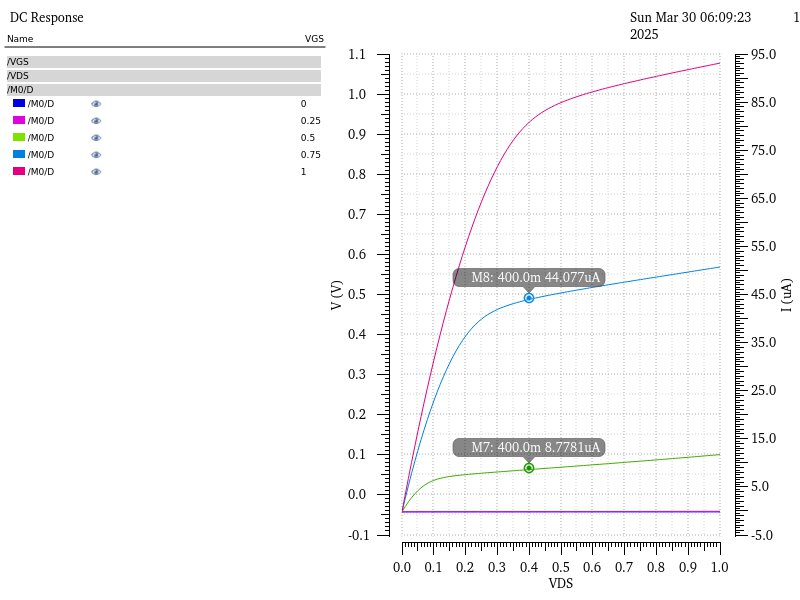
\includegraphics[width=.6\linewidth]{sections/pic/EX3_NMOS_gamma_(w_l)(120_60).png}
	\caption{$I_{DS}$ vs $V_{DS}$ with step $10mV$ with $(W/L) = (120n/60n)$}
	\label{f_EX3_NMOS_gamma_(w_l)(120_60)}
\end{figure}

\[ V_{Th} = \dfrac{V_{GS1} - V_{GS2}\sqrt{\dfrac{I_{DS1}}{I_{DS2}}}}{1 - \sqrt{\dfrac{I_{DS1}}{I_{DS2}}}} = \dfrac{0.75 - 0.5\times \sqrt{\dfrac{44.07\times 10^{-6}}{8.78\times 10^{-6}}}}{1 - \sqrt{\dfrac{44.07\times 10^{-6}}{8.78\times 10^{-6}}}} = 0.3(V)\] 

\[ \gamma = \dfrac{V_{Th} - V_{Th0}}{\sqrt{|2\phi_{F}| + |V_{BS} } - \sqrt{|2\phi_{F}}} = \dfrac{0.3 - 0.13}{\sqrt{0.7 + 0.5} - \sqrt{0.7}} = 0.65 \]

\subsubsection{Measure $k_p$}

\itemmini{For the NMOS transistor with $(W/L) = (90n/50n)$}

\[ k_p = \dfrac{2I_{D}}{\dfrac{L}{W} (V_{GS} - V_{Th0})^{2} (1 + \lambda V_{DS})} = \dfrac{2\times 57.28\times 10^{-6}}{\dfrac{50n}{90n} (0.75 - 0.07)^{2} (1 + 0.52 \times 0.4)} = 317 \times 10^{-6}\]

\itemmini{For the NMOS transistor with $(W/L) = (120n/60n)$}

\[ k_p = \dfrac{2I_{D}}{\dfrac{L}{W} (V_{GS} - V_{Th0})^{2} (1 + \lambda V_{DS})} = \dfrac{2\times 64.21 \times 10^{-6}}{\dfrac{60n}{120n} (0.75 - 0.13)^{2} (1 + 0.44 \times 0.4)} = 568 \times 10^{-6}\]


\subsection{PMOS}

\begin{figure}[H]
	\centering
	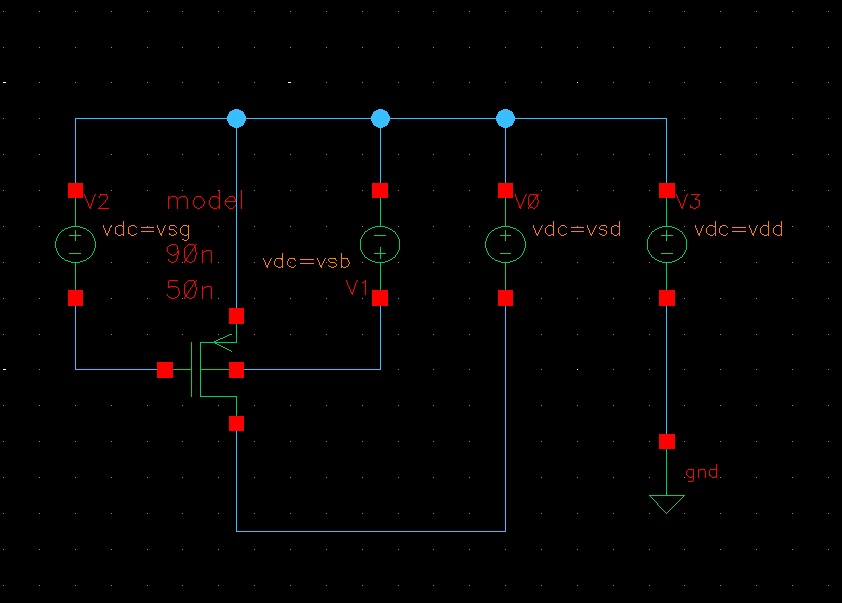
\includegraphics[width = 0.6\linewidth]{sections/pic/EX3_PMOS_schematic.png}
	\caption{Testbench PMOS\_VTG for experiment 3.}
	\label{f_ex3PMOS-schematic}
\end{figure}

\itemmini{Draw curves $I_{D}$ vs $V_{GS}$ @ $V_{DS} = 1V$, $V_{SB} = [0.1, 0.55, 0.9] V$, and sweeping $V_{GS} = [0, 1]V$ with step $10mV$.}

\begin{figure}[H]
	\centering
	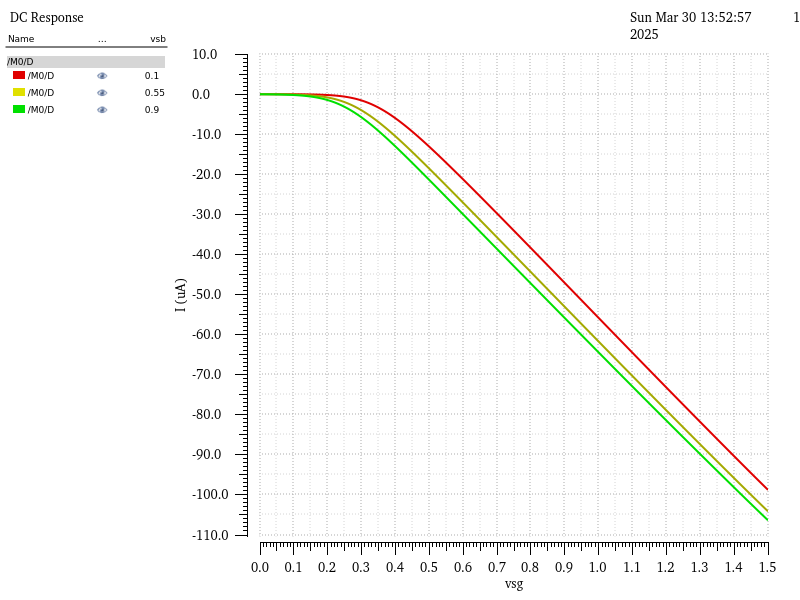
\includegraphics[width=.6\linewidth]{sections/pic/EX3_PMOS_Id&Vgs(Vds=0_1)(w)(l).png}
	\caption{$I_{D}$ vs $V_{GS}$ @ $V_{DS} = 1V$, $V_{SB} = [0.1, 0.55, 0.9] V$, and sweeping $V_{GS} = [0, 1]V$ with step $10mV$.}
	\label{f_EX3_PMOS_Id&Vgs(Vds=0_1)(w)(l)}
\end{figure}

\itemmini{Draw curves $I_{D}$ vs $V_{DS}$ @ $V_{GS} = 1V$, $V_{SB} = [0.1, 0.55, 0.9] V$, and sweeping $V_{DS} = [0, 1]V$ with step $10mV$.}

\begin{figure}[H]
	\centering
	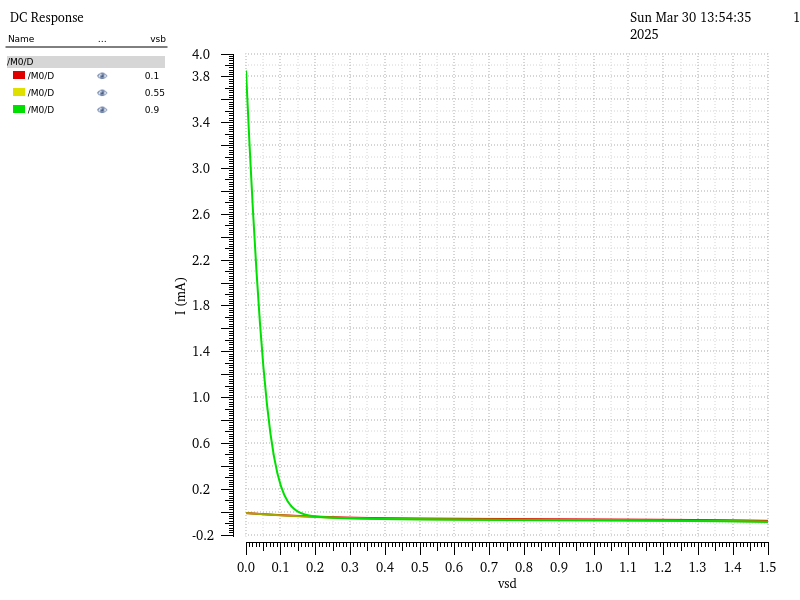
\includegraphics[width=.6\linewidth]{sections/pic/EX3_PMOS_Id&Vds(Vgs=0_1)(w)(l).png}
	\caption{$I_{D}$ vs $V_{DS}$ @ $V_{GS} = 1V$, $V_{SB} = [0.1, 0.55, 0.9] V$, and sweeping $V_{DS} = [0, 1]V$ with step $10mV$.}
	\label{f_EX3_PMOS_Id&Vds(Vgs=0_1)(w)(l)}
\end{figure}


\subsubsection{Measure $\lambda$}
\textbf{Note:} Take points in the saturation region.\\

Draw the curves for $I_{D}$ vs $V_{DS} = [0, 1.5](V)$ with a step of $10mV$, for two values of $V_{GS} = \{0.5, 0.75\}$.\\

\itemmini{For the PMOS transistor with $(W/L) = (90n/50n)$.}

\begin{figure}[H]
	\centering
	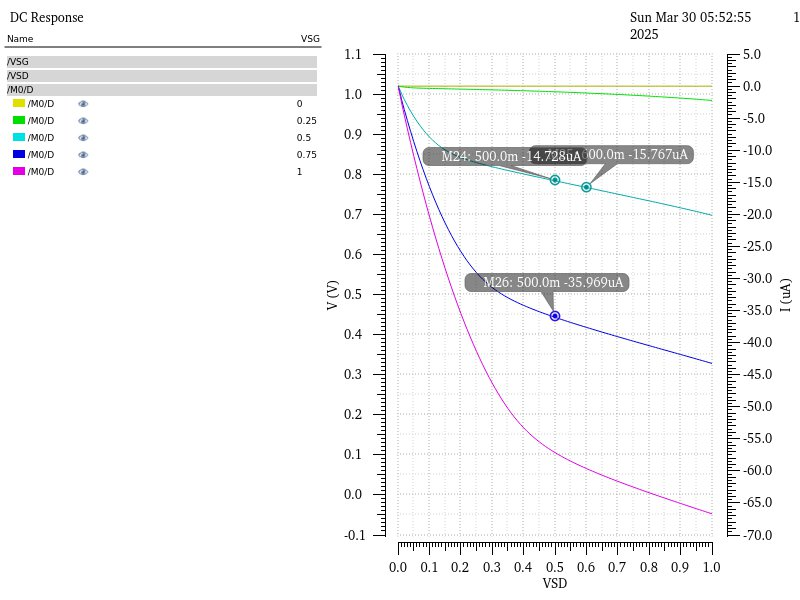
\includegraphics[width=0.6\linewidth]{sections/pic/EX3_PMOS_lambda_(w_l)(90_50).png}
	\caption{$I_{DS}$ vs $V_{DS}$ with step $10mV$ for value of $V_{GS} = 0.5V$ and $(W/L) = (90n/50n)$}
	\label{f_EX3_PMOS_lambda_(w_l)(90_50)}
\end{figure}

\[ \lambda = \dfrac{I_{D2} - I_{D1}}{I_{D1} V_{DS2} - I_{D2} V_{DS1}} \]

With $V_{GS} = 0.5$, we have:

\[ \lambda = \dfrac{I_{D2} - I_{D1}}{I_{D1} V_{DS2} - I_{D2} V_{DS1}} = \dfrac{(-15.77 - -14.73)\times 10^{-6}}{-15.77\times 10^{-6}\times 0.5 - -14.73 \times 10^{-6} \times 0.4 }  = 1.09\]

%Với $V_{GS} = 0.75$ ta có:
%
%\[ \lambda = \dfrac{I_{D2} - I_{D1}}{I_{D1} V_{DS2} - I_{D2} V_{DS1}} = \dfrac{(59.73 - -35.97)\times 10^{-6}}{57.28\times 10^{-6}\times 0.5 - 59.73 \times 10^{-6} \times 0.4 }  = 0.52\]

%Ta thấy $\lambda(0.5)> \lambda(0.75)$. Điều này có nghĩa là khi $V_{GS}$ thấp, độ ổn định của $I_{DS}$ trong vùng bão hòa kém hơn.\\ 

\itemmini{For the PMOS transistor with $(W/L) = (120n/60n)$.}

\begin{figure}[H]
	\centering
	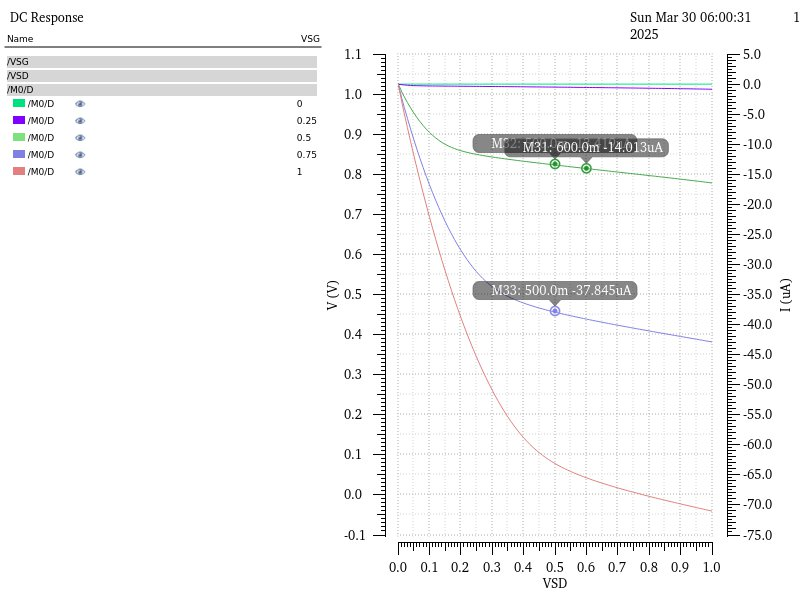
\includegraphics[width=.6\linewidth]{sections/pic/EX3_PMOS_lambda_(w_l)(120_90)(vgs_0_5).png}
	\caption{$I_{DS}$ vs $V_{DS}$ with step $10mV$  for value of $V_{GS} = 0.5$ and $(W/L) = (120n/60n)$}
	\label{f_EX3_PMOS_lambda_(w_l)(120_90)(vgs_0_5)}
\end{figure}

With $V_{GS} = 0.5$, we have:

\[ \lambda = \dfrac{I_{D2} - I_{D1}}{I_{D1} V_{DS2} - I_{D2} V_{DS1}} = \dfrac{(-14.01 - -13.41)\times 10^{-6}}{-13.41\times 10^{-6}\times 0.5 - -14.01 \times 10^{-6} \times 0.4 }  = 0.576 \]

%Vậy khi PMOS có công nghệ càng nhỏ thì $\lambda$ càng tăng. Lý do là khi $L$ giảm, hiệu ứng \textit{Chiều dài kênh ngắn (SCE - Short Channel Effect)} trở nên rõ nệt hơn, làm tăng sự phụ thuộc của $I_{DS}$ và $V_{DS}$. Điều này khiến cho hệ số $\lambda$ tăng lên, nghĩa là $I_{DS}$ kém ổn định hơn.

\subsubsection{Measure $V_{Th0}$}
\[ V_{Th} = \dfrac{V_{GS1} - V_{GS2}\sqrt{\dfrac{I_{DS1}}{I_{DS2}}}}{1 - \sqrt{\dfrac{I_{DS1}}{I_{DS2}}}} \]

\itemmini{For the PMOS transistor with $(W/L) = (90n/50n)$.}

\begin{figure}[H]
	\centering
	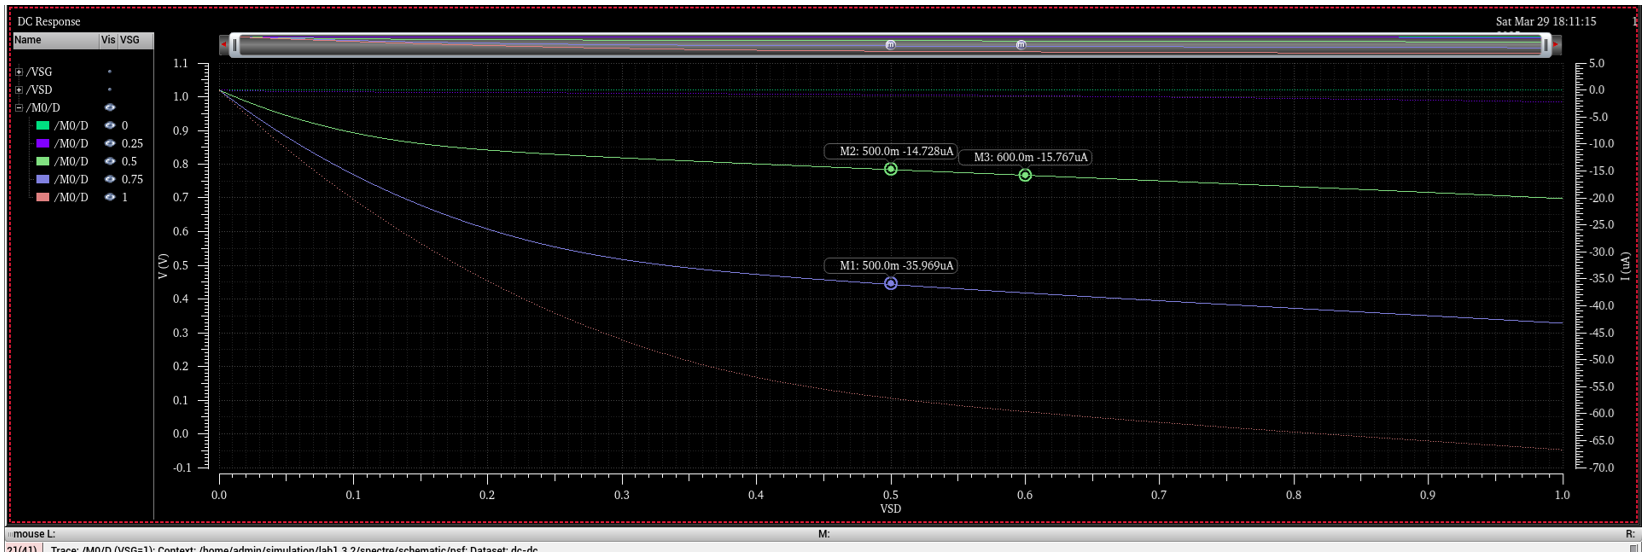
\includegraphics[width=.6\linewidth]{sections/pic/EX3_PMOS_vth0_(w_l)(90_50).png}
	\caption{$I_{DS}$ vs $V_{DS}$ with step $10mV$ for $(W/L) = (90n/50n)$}
	\label{f_EX3_PMOS_vth0_(w_l)(90_50)}
\end{figure}

\[ V_{Th0} = \dfrac{V_{GS1} - V_{GS2}\sqrt{\dfrac{I_{DS1}}{I_{DS2}}}}{1 - \sqrt{\dfrac{I_{DS1}}{I_{DS2}}}} = \dfrac{0.75 - 0.5\times \sqrt{\dfrac{-35.97\times 10^{-6}}{-14.73\times 10^{-6}}}}{1 - \sqrt{\dfrac{-35.79\times 10^{-6}}{-14.73\times 10^{-6}}}} = 0.056(V)\]

\itemmini{For the PMOS transistor with $(W/L) = (120n/60n)$.}

\begin{figure}[H]
	\centering
	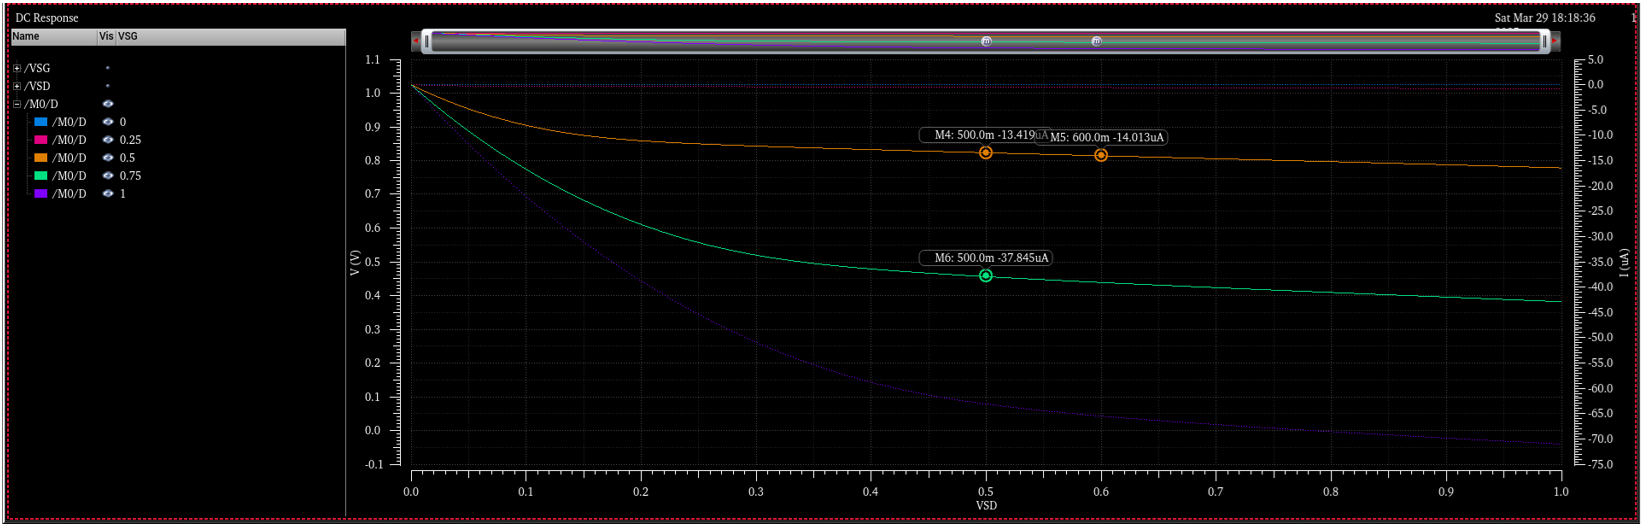
\includegraphics[width=.6\linewidth]{sections/pic/EX3_PMOS_vth0_(w_l)(120_60).png}
	\caption{$I_{DS}$ vs $V_{DS}$ with step $10mV$ for $(W/L) = (120n/60n)$}
	\label{f_EX3_PMOS_vth0_(w_l)(120_60)}
\end{figure}

\[ V_{Th0} = \dfrac{V_{GS1} - V_{GS2}\sqrt{\dfrac{I_{DS1}}{I_{DS2}}}}{1 - \sqrt{\dfrac{I_{DS1}}{I_{DS2}}}} = \dfrac{0.75 - 0.5\times \sqrt{\dfrac{-37.85\times 10^{-6}}{-13.42\times 10^{-6}}}}{1 - \sqrt{\dfrac{-37.85\times 10^{-6}}{-13.42\times 10^{-6}}}} = 0.132(V)\] 


%KHi tỷ lệ $W/L$ thay đổi, $VTH$ có thể bị ảnh hưởng do hiệu ứng \textit{Chiều dài kênh ngắn (SCE)}.
%
%Khi $L$ giảm (trong trường hợp PMOS $90n/50n$), $VTH$ có xu hướng giảm do hiệu ứng kéo rào thế xuống (DIBL - Drain-Induced Barrier Lowering).
%
%Khi $L$ lớn hơn (trong trường hợp PMOS $120n/60n$), $VTH$ cao hơn vì hiệu ứng chiều dài kênh ngắn ít rõ rệt hơn.

\subsubsection{Measure $\gamma$}

\itemmini{For the PMOS transistor with $(W/L) = (90n/50n)$ và $V_{BS} = 0.5$.}

\begin{figure}[H]
	\centering
	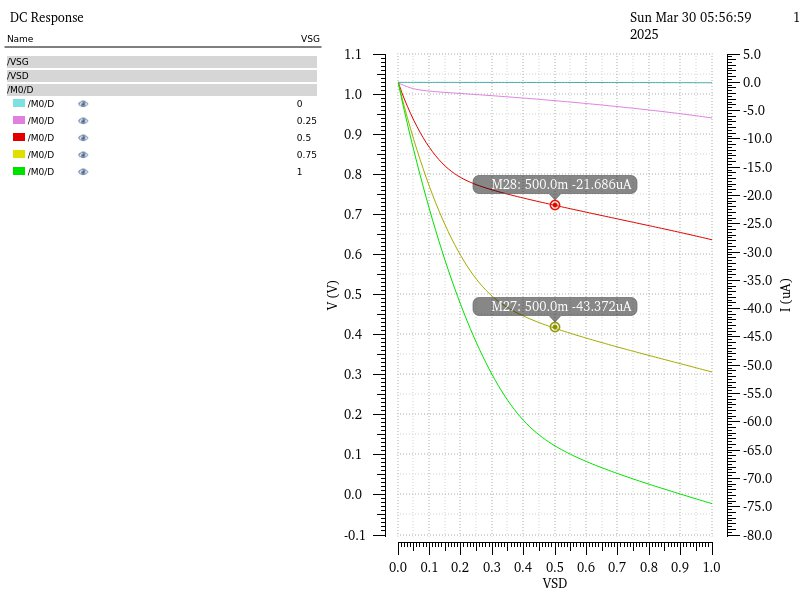
\includegraphics[width=.6\linewidth]{sections/pic/EX3_PMOS_gamma_(w_l)(90_50).png}
	\caption{$I_{DS}$ vs. $V_{DS}$ with a step of $10,\text{mV}$ for $(W/L) = (90n/50n)$}
	\label{f_EX3_PMOS_gamma_(w_l)(90_50)}
\end{figure}

\[ V_{Th} = \dfrac{V_{GS1} - V_{GS2}\sqrt{\dfrac{I_{DS1}}{I_{DS2}}}}{1 - \sqrt{\dfrac{I_{DS1}}{I_{DS2}}}} = \dfrac{0.75 - 0.5\times \sqrt{\dfrac{-43.37\times 10^{-6}}{-21.68\times 10^{-6}}}}{1 - \sqrt{\dfrac{-43.37\times 10^{-6}}{-21.68\times 10^{-6}}}} = -0.103(V)\] 


We have, $2\phi F = 0.7 \gamma$:

\[ \gamma = \dfrac{V_{Th} - V_{Th0}}{\sqrt{|2\phi_{F}| + |V_{BS} } - \sqrt{|2\phi_{F}}} = \dfrac{-0.103 - 0.056}{\sqrt{0.7 + 0.5} - \sqrt{0.7}} =-0.182 \]

%Vậy ta có thể kết luận khi $\gamma$ tăng khiến $V_{Th}$ tăng mạnh hơn khi $V_{BS}$ tăng.\\
When $V_{BS}$ increases, the $V_{Th}$ of PMOS typically rises, but the extent of this change depends on the sign of $\gamma$ and the fabrication technology.\\

\itemmini{For the PMOS transistor with $(W/L) = (120n/60n)$ and $V_{BS} = 0.5$.}

\begin{figure}[H]
	\centering
	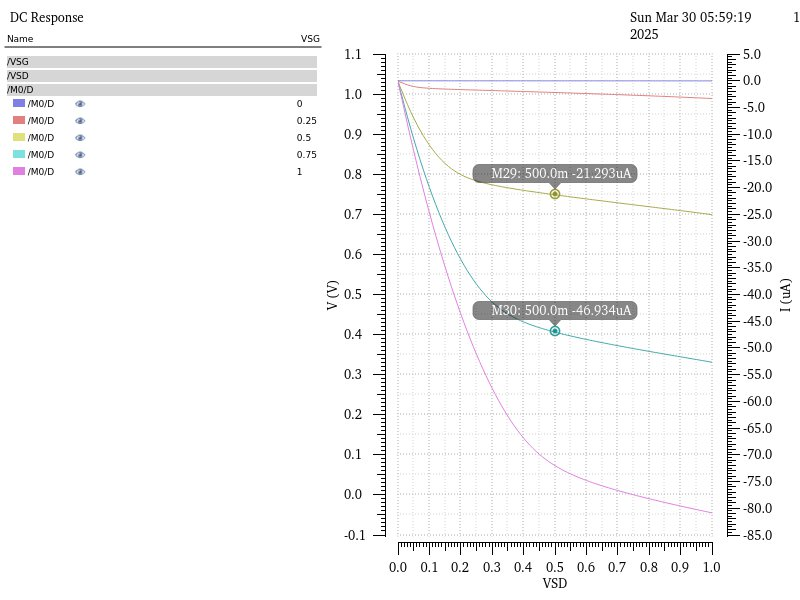
\includegraphics[width=.6\linewidth]{sections/pic/EX3_PMOS_gamma_(w_l)(120_60).png}
	\caption{$I_{DS}$ vs $V_{DS}$ with step $10mV$ với $(W/L) = (120n/60n)$}
	\label{f_EX3_PMOS_gamma_(w_l)(120_60)}
\end{figure}

\[ V_{Th} = \dfrac{V_{GS1} - V_{GS2}\sqrt{\dfrac{I_{DS1}}{I_{DS2}}}}{1 - \sqrt{\dfrac{I_{DS1}}{I_{DS2}}}} = \dfrac{0.75 - 0.5\times \sqrt{\dfrac{-46.93\times 10^{-6}}{-21.29\times 10^{-6}}}}{1 - \sqrt{\dfrac{-46.93\times 10^{-6}}{-21.29\times 10^{-6}}}} = -0.016(V)\] 

\[ \gamma = \dfrac{V_{Th} - V_{Th0}}{\sqrt{|2\phi_{F}| + |V_{BS} } - \sqrt{|2\phi_{F}}} = \dfrac{-0.016 - 0.132}{\sqrt{0.7 + 0.5} - \sqrt{0.7}} = -0.572 \]

\subsubsection{Measure $k_p$}

\itemmini{For the PMOS transistor with $(W/L) = (90n/50n)$}

\[ k_p = \dfrac{2I_{D}}{\dfrac{L}{W} (V_{GS} - V_{Th0})^{2} (1 + \lambda V_{DS})} = \dfrac{2\times -14.73 \times 10^{-6}}{\dfrac{50n}{90n} (0.5 - 0.056)^{2} (1 + 0.5 \times 1.09)} = -174 \times 10^{-6}\]

\itemmini{For the PMOS transistor with $(W/L) = (120n/60n)$}

\[ k_p = \dfrac{2I_{D}}{\dfrac{L}{W} (V_{GS} - V_{Th0})^{2} (1 + \lambda V_{DS})} = \dfrac{2\times -13.42 \times 10^{-6}}{\dfrac{60n}{120n} (0.5 - 0.132)^{2} (1 + 0.576 \times 0.5)} = -308 \times 10^{-6}\]


